% Generated by LitigCharts.PublicationFigures. Captions and provenance are sidecars.
\documentclass[10pt,tikz,border=5pt]{standalone}
\usepackage{lmodern}
\usetikzlibrary{patterns,patterns.meta}
\begin{document}
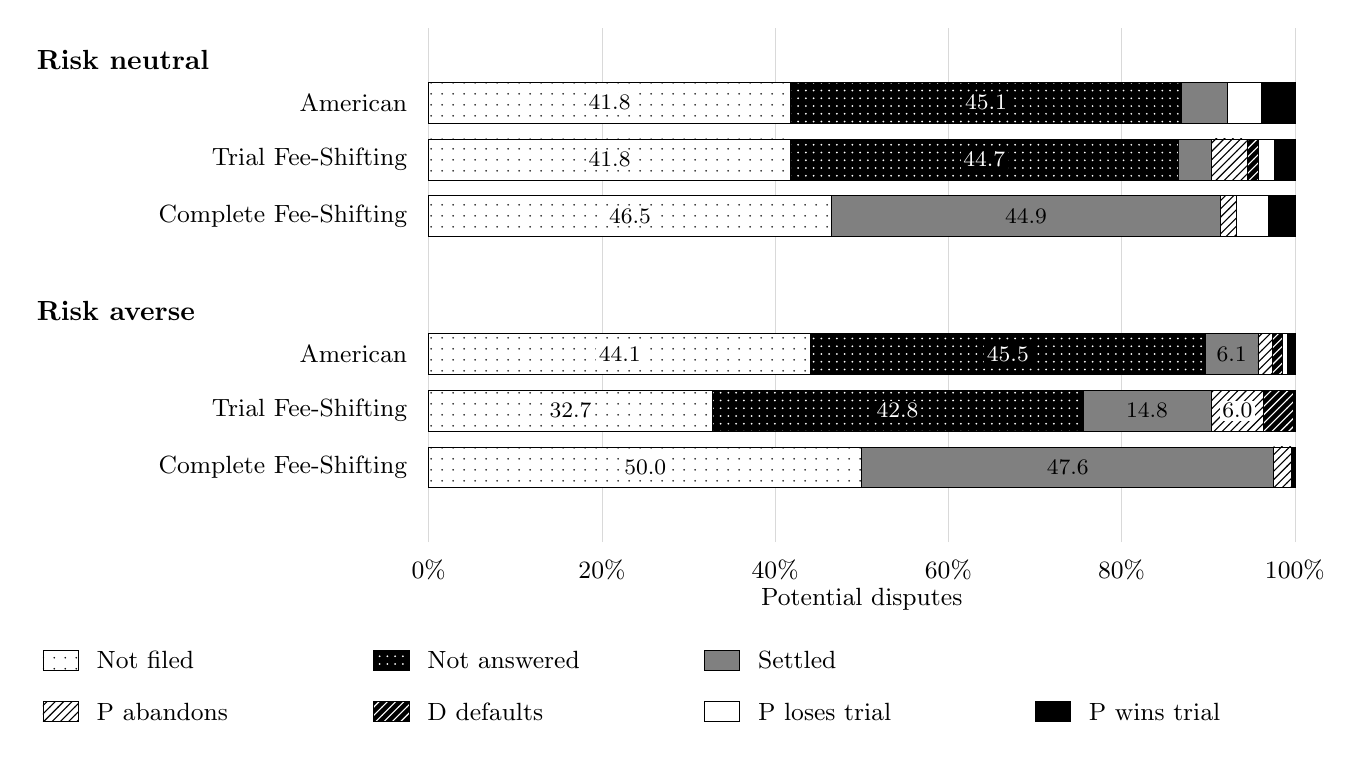
\begin{tikzpicture}[font=\small]\draw[black!15,line width=.2pt] (5.1,.65) -- (5.1,7.18);
\node[anchor=north] at (5.1,.55) {0\%};
\draw[black!15,line width=.2pt] (7.3,.65) -- (7.3,7.18);
\node[anchor=north] at (7.3,.55) {20\%};
\draw[black!15,line width=.2pt] (9.5,.65) -- (9.5,7.18);
\node[anchor=north] at (9.5,.55) {40\%};
\draw[black!15,line width=.2pt] (11.7,.65) -- (11.7,7.18);
\node[anchor=north] at (11.7,.55) {60\%};
\draw[black!15,line width=.2pt] (13.9,.65) -- (13.9,7.18);
\node[anchor=north] at (13.9,.55) {80\%};
\draw[black!15,line width=.2pt] (16.1,.65) -- (16.1,7.18);
\node[anchor=north] at (16.1,.55) {100\%};
\node[anchor=west,font=\bfseries] at (0,6.78) {\mbox{Risk} \mbox{neutral}};
\node[anchor=east] at (4.95,6.23) {American};
\path[preaction={fill=white,draw=none},pattern={Dots[distance=4pt,radius=.35pt]},pattern color=black,draw=black,line width=.25pt] (5.1,5.97) rectangle (9.69503,6.49);
\node[text=black,fill=white,font=\footnotesize,inner sep=1pt] at (7.397515,6.23) {41.8};
\path[preaction={fill=black,draw=none},pattern={Dots[distance=2.8pt,radius=.35pt]},pattern color=white,draw=black,line width=.25pt] (9.69503,5.97) rectangle (14.661222,6.49);
\node[text=white,fill=black,font=\footnotesize,inner sep=1pt] at (12.178126,6.23) {45.1};
\path[fill=black!50,draw=black,line width=.25pt] (14.661222,5.97) rectangle (15.246984,6.49);
\path[fill=white,draw=black,line width=.25pt] (15.246984,5.97) rectangle (15.669418,6.49);
\path[fill=black,draw=black,line width=.25pt] (15.669418,5.97) rectangle (16.100004,6.49);
\node[anchor=east] at (4.95,5.51) {Trial Fee-Shifting};
\path[preaction={fill=white,draw=none},pattern={Dots[distance=4pt,radius=.35pt]},pattern color=black,draw=black,line width=.25pt] (5.1,5.25) rectangle (9.69503,5.77);
\node[text=black,fill=white,font=\footnotesize,inner sep=1pt] at (7.397515,5.51) {41.8};
\path[preaction={fill=black,draw=none},pattern={Dots[distance=2.8pt,radius=.35pt]},pattern color=white,draw=black,line width=.25pt] (9.69503,5.25) rectangle (14.61654,5.77);
\node[text=white,fill=black,font=\footnotesize,inner sep=1pt] at (12.155785,5.51) {44.7};
\path[fill=black!50,draw=black,line width=.25pt] (14.61654,5.25) rectangle (15.043759,5.77);
\path[preaction={fill=white,draw=none},pattern={north east lines},pattern color=black,draw=black,line width=.25pt] (15.043759,5.25) rectangle (15.491477,5.77);
\path[preaction={fill=black,draw=none},pattern={north east lines},pattern color=white,draw=black,line width=.25pt] (15.491477,5.25) rectangle (15.6393,5.77);
\path[fill=white,draw=black,line width=.25pt] (15.6393,5.25) rectangle (15.840245,5.77);
\path[fill=black,draw=black,line width=.25pt] (15.840245,5.25) rectangle (16.100003,5.77);
\node[anchor=east] at (4.95,4.79) {Complete Fee-Shifting};
\path[preaction={fill=white,draw=none},pattern={Dots[distance=4pt,radius=.35pt]},pattern color=black,draw=black,line width=.25pt] (5.1,4.53) rectangle (10.214758,5.05);
\node[text=black,fill=white,font=\footnotesize,inner sep=1pt] at (7.657379,4.79) {46.5};
\path[fill=black!50,draw=black,line width=.25pt] (10.214758,4.53) rectangle (15.157905,5.05);
\node[text=black,fill=none,font=\footnotesize,inner sep=1pt] at (12.686332,4.79) {44.9};
\path[preaction={fill=white,draw=none},pattern={north east lines},pattern color=black,draw=black,line width=.25pt] (15.157905,4.53) rectangle (15.358234,5.05);
\path[fill=white,draw=black,line width=.25pt] (15.358234,4.53) rectangle (15.759057,5.05);
\path[fill=black,draw=black,line width=.25pt] (15.759057,4.53) rectangle (16.099995,5.05);
\node[anchor=west,font=\bfseries] at (0,3.59) {\mbox{Risk} \mbox{averse}};
\node[anchor=east] at (4.95,3.04) {American};
\path[preaction={fill=white,draw=none},pattern={Dots[distance=4pt,radius=.35pt]},pattern color=black,draw=black,line width=.25pt] (5.1,2.78) rectangle (9.950626,3.3);
\node[text=black,fill=white,font=\footnotesize,inner sep=1pt] at (7.525313,3.04) {44.1};
\path[preaction={fill=black,draw=none},pattern={Dots[distance=2.8pt,radius=.35pt]},pattern color=white,draw=black,line width=.25pt] (9.950626,2.78) rectangle (14.960521,3.3);
\node[text=white,fill=black,font=\footnotesize,inner sep=1pt] at (12.455574,3.04) {45.5};
\path[fill=black!50,draw=black,line width=.25pt] (14.960521,2.78) rectangle (15.631851,3.3);
\node[text=black,fill=none,font=\footnotesize,inner sep=1pt] at (15.296186,3.04) {6.1};
\path[preaction={fill=white,draw=none},pattern={north east lines},pattern color=black,draw=black,line width=.25pt] (15.631851,2.78) rectangle (15.813438,3.3);
\path[preaction={fill=black,draw=none},pattern={north east lines},pattern color=white,draw=black,line width=.25pt] (15.813438,2.78) rectangle (15.936387,3.3);
\path[fill=white,draw=black,line width=.25pt] (15.936387,2.78) rectangle (16.003346,3.3);
\path[fill=black,draw=black,line width=.25pt] (16.003346,2.78) rectangle (16.099995,3.3);
\node[anchor=east] at (4.95,2.32) {Trial Fee-Shifting};
\path[preaction={fill=white,draw=none},pattern={Dots[distance=4pt,radius=.35pt]},pattern color=black,draw=black,line width=.25pt] (5.1,2.06) rectangle (8.700245,2.58);
\node[text=black,fill=white,font=\footnotesize,inner sep=1pt] at (6.900123,2.32) {32.7};
\path[preaction={fill=black,draw=none},pattern={Dots[distance=2.8pt,radius=.35pt]},pattern color=white,draw=black,line width=.25pt] (8.700245,2.06) rectangle (13.408036,2.58);
\node[text=white,fill=black,font=\footnotesize,inner sep=1pt] at (11.054141,2.32) {42.8};
\path[fill=black!50,draw=black,line width=.25pt] (13.408036,2.06) rectangle (15.03872,2.58);
\node[text=black,fill=none,font=\footnotesize,inner sep=1pt] at (14.223378,2.32) {14.8};
\path[preaction={fill=white,draw=none},pattern={north east lines},pattern color=black,draw=black,line width=.25pt] (15.03872,2.06) rectangle (15.703267,2.58);
\node[text=black,fill=white,font=\footnotesize,inner sep=1pt] at (15.370994,2.32) {6.0};
\path[preaction={fill=black,draw=none},pattern={north east lines},pattern color=white,draw=black,line width=.25pt] (15.703267,2.06) rectangle (16.077861,2.58);
\path[fill=white,draw=black,line width=.25pt] (16.077861,2.06) rectangle (16.090115,2.58);
\path[fill=black,draw=black,line width=.25pt] (16.090115,2.06) rectangle (16.100003,2.58);
\node[anchor=east] at (4.95,1.6) {Complete Fee-Shifting};
\path[preaction={fill=white,draw=none},pattern={Dots[distance=4pt,radius=.35pt]},pattern color=black,draw=black,line width=.25pt] (5.1,1.34) rectangle (10.6,1.86);
\node[text=black,fill=white,font=\footnotesize,inner sep=1pt] at (7.85,1.6) {50.0};
\path[fill=black!50,draw=black,line width=.25pt] (10.6,1.34) rectangle (15.830775,1.86);
\node[text=black,fill=none,font=\footnotesize,inner sep=1pt] at (13.215388,1.6) {47.6};
\path[preaction={fill=white,draw=none},pattern={north east lines},pattern color=black,draw=black,line width=.25pt] (15.830775,1.34) rectangle (16.058868,1.86);
\path[fill=white,draw=black,line width=.25pt] (16.058868,1.34) rectangle (16.06783,1.86);
\path[fill=black,draw=black,line width=.25pt] (16.06783,1.34) rectangle (16.1,1.86);
\node at (10.6,-.08) {Potential disputes};
\path[preaction={fill=white,draw=none},pattern={Dots[distance=4pt,radius=.35pt]},pattern color=black,draw=black,line width=.25pt] (0.2,-0.98) rectangle (0.65,-0.72);
\node[anchor=west] at (0.76,-0.85) {Not filed};
\path[preaction={fill=black,draw=none},pattern={Dots[distance=2.8pt,radius=.35pt]},pattern color=white,draw=black,line width=.25pt] (4.4,-0.98) rectangle (4.85,-0.72);
\node[anchor=west] at (4.96,-0.85) {Not answered};
\path[fill=black!50,draw=black,line width=.25pt] (8.6,-0.98) rectangle (9.05,-0.72);
\node[anchor=west] at (9.16,-0.85) {Settled};
\path[preaction={fill=white,draw=none},pattern={north east lines},pattern color=black,draw=black,line width=.25pt] (0.2,-1.63) rectangle (0.65,-1.37);
\node[anchor=west] at (0.76,-1.5) {P abandons};
\path[preaction={fill=black,draw=none},pattern={north east lines},pattern color=white,draw=black,line width=.25pt] (4.4,-1.63) rectangle (4.85,-1.37);
\node[anchor=west] at (4.96,-1.5) {D defaults};
\path[fill=white,draw=black,line width=.25pt] (8.6,-1.63) rectangle (9.05,-1.37);
\node[anchor=west] at (9.16,-1.5) {P loses trial};
\path[fill=black,draw=black,line width=.25pt] (12.8,-1.63) rectangle (13.25,-1.37);
\node[anchor=west] at (13.36,-1.5) {P wins trial};
\end{tikzpicture}
\end{document}
